\documentclass[12pt]{article}
\usepackage[margin=0.75in]{geometry}
\usepackage{microtype}
\usepackage{amsmath,amssymb}
\usepackage{array,delarray}
\usepackage[dvips]{graphicx} \usepackage{xspace}
\usepackage{wrapfig}
\usepackage{color}
\usepackage[square,sort&compress,numbers]{natbib}
\usepackage{times}
%\usepackage{caption}
\usepackage{subfig}
%\usepackage{subcaption}
\usepackage{colortbl}
\usepackage[table]{xcolor}
\usepackage{url}
\usepackage{microtype}
\usepackage{nomencl}

\usepackage{hyperref}
\hypersetup{colorlinks=true,linkcolor=blue,linkcolor=blue,citecolor=blue,urlcolor=blue}

%%
\graphicspath{{./}{./figs/}}

%%\usepackage{citesort}
%\usepackage{sidecap}
%\usepackage{times} % assumes new font selection scheme installed
%\usepackage[small]{caption}




\renewcommand{\thesection}{\Roman{section}}
\renewcommand{\thesubsection}{{\bfseries\Alph{subsection}}}

\DeclareMathOperator*{\argmin}{arg\,min}



\title{Creating synthetic distribution networks}



%%
\begin{document}
	\maketitle
	
	\section{Algorithm}
\subsection{Constructing the mapping}\label{subsec:map}
\begin{figure}
	\centering
	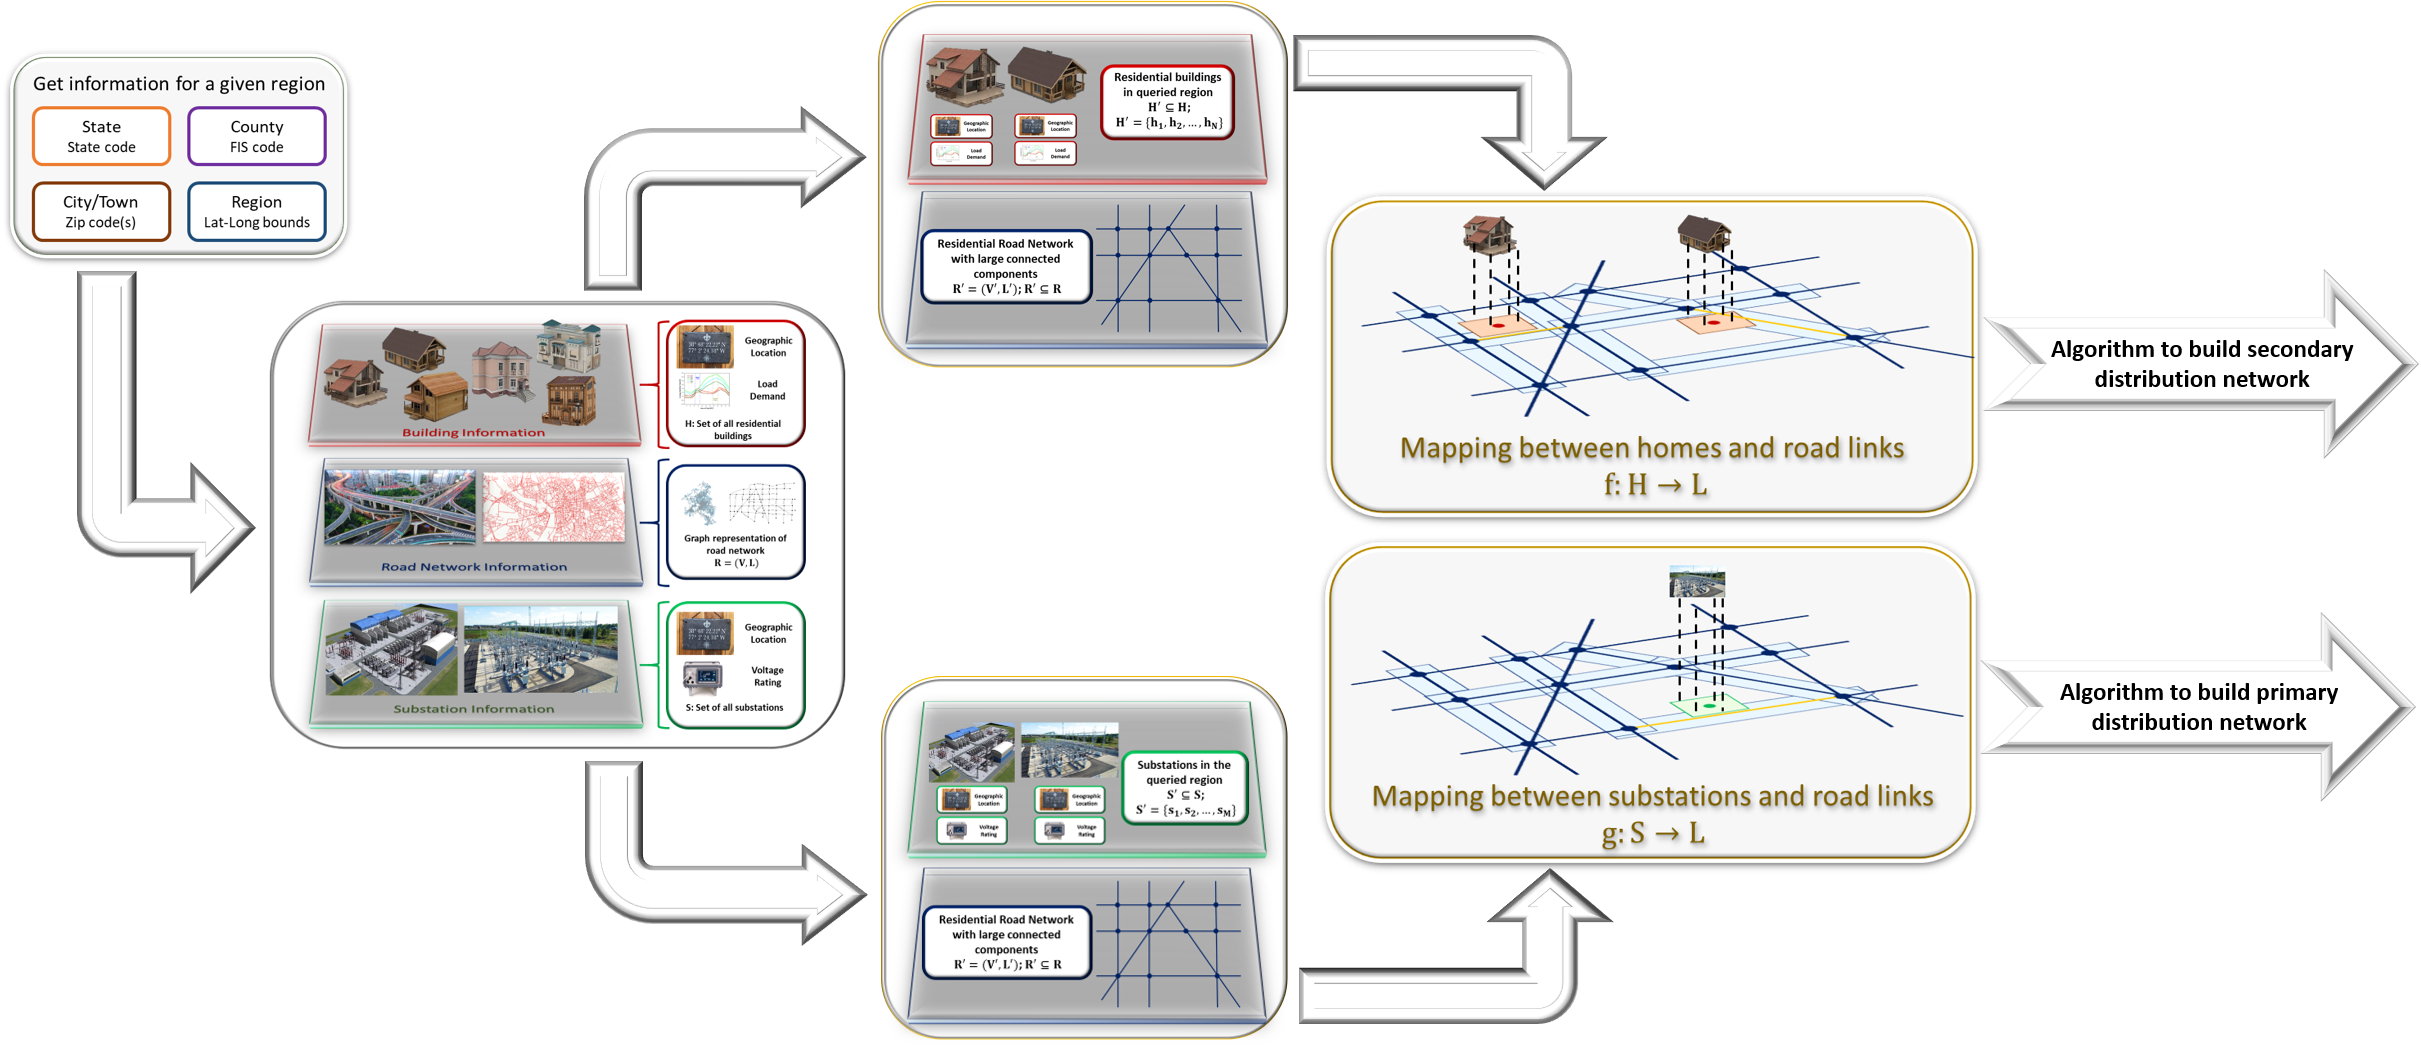
\includegraphics[scale=0.42]{pipeline_1}
	\caption{Flowchart showing the generation of maps between three data sets.}
\end{figure}
\begin{algorithm}[H]
	\caption{Find the nearest link in $\mathsf{L}$ to a given point $\mathbf{p}$.}
	\label{alg:dist}
	\begin{algorithmic}[1]
		\Require Radius for bounding boxes $r$, a mapping $\mathsf{dist}:\mathbb{R}^2\times\mathsf{L}\rightarrow\mathbb{R}^{+}$ such that $\mathsf{dist}(\mathbf{p},\mathbf{l})$ is the shortest distance between point $\mathbf{p}\in\mathbb{R}^2$ and link segment $\mathbf{l}=\mathbf{u}-\mathbf{v}$ for $\mathbf{l}\in\mathsf{L}$ and $\mathbf{u},\mathbf{v}\in\mathbb{R}^2$.
		\For {each link $\mathbf{l}\in\mathsf{L}$}
		\State evaluate bounding box $\mathbf{B_l}$ such that $\mathbf{B_l}=\big\{\mathbf{x}\big|||\mathbf{x}-\mathbf{x_l}||_2\leq r,\forall \mathbf{x_l}=\theta\mathbf{u}+(1-\theta)\mathbf{v},\theta=[0,1]\big\}$.
		\EndFor
		\State Evaluate bounding box $\mathbf{B_p}$ for point $\mathbf{p}$ such that $\mathbf{B_l}=\big\{\mathbf{x}\big|||\mathbf{x}-\mathbf{p}||_2\leq r\big\}$.
		\State Find the bounding boxes $\mathbf{B_{l_1}},\mathbf{B_{l_2}},\cdots,\mathbf{B_{l_m}}$ which intersect with $\mathbf{B_p}$.
		\State Find the link $\mathbf{l^\star}\in\mathsf{L'}$, where $\mathsf{L'}=\{\mathbf{l_1},\mathbf{l_2},\cdots,\mathbf{l_m}\}\subseteq\mathsf{L}$ such that $\mathbf{l^\star}=\argmin_{\mathbf{l}\in\mathsf{L}}\mathsf{dist}(\mathbf{p},\mathbf{l})$.
	\end{algorithmic}
\end{algorithm}
\begin{algorithm}[H]
	\caption{Generate mapping between building and road network data sets.}
	\label{alg:map1}
	\begin{algorithmic}[1]
		\Require Road network graph $\mathsf{R=(\mathsf{V},\mathsf{L})}$, set of residential buildings $\mathsf{H}$, a mapping $\mathsf{dist}:\mathsf{H}\times\mathsf{V}\rightarrow\mathbb{R}^{+}$ such that $\mathsf{dist}(h,v)$ is the Euclidean distance between building $h\in\mathsf{H}$ and road network node $v\in\mathsf{V}$.
		\Initialize :A mapping from road nodes to set of sets of buildings $p:\mathsf{V}\rightarrow\mathcal{H}$ such that $p(v)=\emptyset,\forall v\in\mathsf{V}$
		\For {each building $h\in\mathsf{H}$}
		\State find mapping $f:\mathsf{H}\rightarrow\mathsf{L}$ using Algorithm~\ref{alg:dist} to generate the nearest link $e\in\mathsf{L}$.
		\EndFor
		\For {each link $e=(u,v)\in\mathsf{L}$}
		\State Initialize four sets: $\mathsf{H_{uA}},\mathsf{H_{vA}},\mathsf{H_{uB}},\mathsf{H_{vB}}=\emptyset$.
		\State find the inverse mapping $f^{-1}:\mathsf{L}\rightarrow\mathsf{H}$ which generates the set of buildings $\mathsf{H_e}$ associated with $e$.
		\State find the set of buildings $\mathsf{H_{eA}},\mathsf{H_{eB}}\subseteq\mathsf{H_e}$ with $\mathsf{H_{eA}}\cup\mathsf{H_{eB}}=\mathsf{H_e}$ which are on opposite sides of $e$.
		\For {each building $h\in\mathsf{H_{eA}}$}
		\If {$\mathsf{dist}(h,u)<\mathsf{dist}(h,v)$}
		\State Add this building to set $\mathsf{H_{uA}}$: $\mathsf{H_{uA}}\leftarrow\mathsf{H_{uA}}\cup\{h\}$
		\Else
		\State Add this building to set $\mathsf{H_{vA}}$: $\mathsf{H_{vA}}\leftarrow\mathsf{H_{vA}}\cup\{h\}$
		\EndIf
		\EndFor
		\For {each building $h\in\mathsf{H_{eB}}$}
		\If {$\mathsf{dist}(h,u)<\mathsf{dist}(h,v)$}
		\State Add this building to set $\mathsf{H_{uB}}$: $\mathsf{H_{uB}}\leftarrow\mathsf{H_{uB}}\cup\{h\}$
		\Else
		\State Add this building to set $\mathsf{H_{vB}}$: $\mathsf{H_{vB}}\leftarrow\mathsf{H_{vB}}\cup\{h\}$
		\EndIf
		\EndFor
		\State Add the sets $\mathsf{H_{uA}},\mathsf{H_{uB}}$ to the mapping $p(u)$: $p(u)\leftarrow p(u)\cup\{\mathsf{H_{uA}},\mathsf{H_{uB}}\}$.
		\State Add the sets $\mathsf{H_{vA}},\mathsf{H_{vB}}$ to the mapping $p(v)$: $p(v)\leftarrow p(v)\cup\{\mathsf{H_{vA}},\mathsf{H_{vB}}\}$.
		\EndFor
	\end{algorithmic}
\end{algorithm}

\begin{algorithm}[H]
	\caption{Generate mapping between substations and road network nodes.}
	\label{alg:map2}
	\begin{algorithmic}[1]
		\Require Road network graph $\mathsf{R=(\mathsf{V},\mathsf{L})}$, set of substations $\mathsf{S}$, a mapping $\mathsf{dist}:\mathsf{S}\times\mathsf{V}\rightarrow\mathbb{R}^{+}$ such that $\mathsf{dist}(s,v)$ is the Euclidean distance between substation $s\in\mathsf{S}$ and road network node $v\in\mathsf{V}$, mapping $p:\mathsf{V}\rightarrow\mathcal{H}$ obtained from Algorithm~\ref{alg:map1}, minimum number of road network nodes mapped to a substation $N_{min}$.
		\For {each road network node $v\in\mathsf{V}$}
		\If {$p(v)=\emptyset$}
		\State Remove node $v$ from set of all road network nodes $\mathsf{V}\leftarrow\mathsf{V}\setminus\{v\}$.
		\Else 
		\State Find a mapping $g:\mathsf{V}\rightarrow\mathsf{S}$ which identifies the nearest substation to the road node $v$ such that $g(v)=\argmin_{s\in\mathsf{S}}\mathsf{dist}(s,v)$.
		\EndIf
		\EndFor
		\For {each substation $s\in\mathsf{S}$}
		\State Find inverse mapping $g^{-1}:\mathsf{S}\rightarrow\mathsf{V}$ which generates the set of road network nodes $\mathsf{V_s}$ associated with $s$.
		\If {$|g^{-1}(s)|<N_{min}$}
		\State Remove the substation from set of all substations, $\mathsf{S}\leftarrow\mathsf{S}\setminus\{s\}$
		\EndIf 
		\EndFor
		\State Recompute mapping $g:\mathsf{V}\rightarrow\mathsf{S}$ which identifies the nearest substation to the road node $v$ such that $g(v)=\argmin_{s\in\mathsf{S}}\mathsf{dist}(s,v)$.
	\end{algorithmic}
\end{algorithm}

\begin{figure}[H]
	\centering
	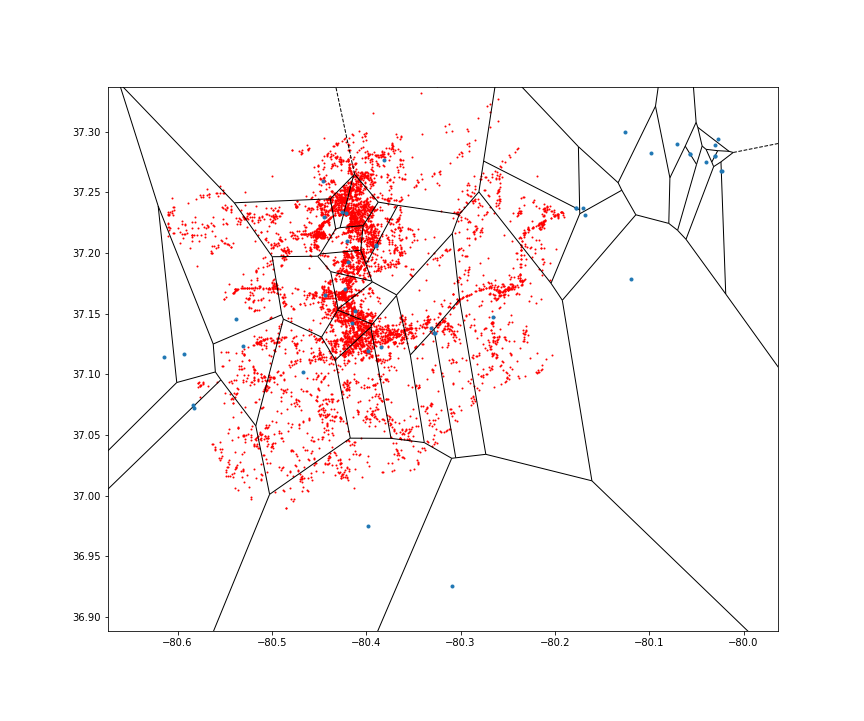
\includegraphics[scale=0.42]{map1}
	\caption{Voronoi regions formed by substations (blue points) and the road nodes (red points) mapped within each region. A number of substations have very road nodes associated with it. Therefore, the Voronoi regions are recomputed after removing the unmapped substations.}
\end{figure}

\begin{figure}[H]
	\centering
	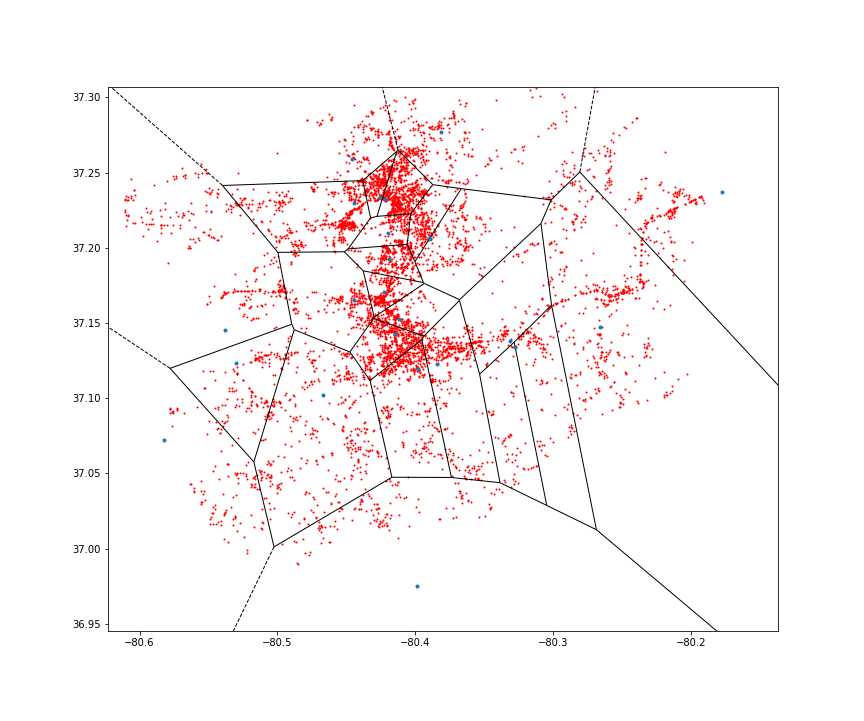
\includegraphics[scale=0.42]{map2}
	\caption{Voronoi regions formed by substations (blue points) and the road nodes (red points) mapped within each region. Almost all the regions are densely distributed by road network nodes. The boundary regions seem to be empty. However, they would be filled by road nodes from the neighboring counties.}
\end{figure}

	\section{Problem Formulation}
Using the mapping proposed in the previous section, we can consider nodes in the road network to be nodes in the distribution grid. Let $\mathsf{\Omega_b}$ denote the set of all nodes in the road network along with the substation buses. Let $\mathsf{\Omega_{bs}}\subset\mathsf{\Omega_b}$ denote the set of substation buses. Furthermore, the mapping $p^{-1}$ between road nodes and activity locations can be used to evaluate the load demand at each node. Let $P_{Di}$ and $P_{Si}$ denote the load and power supplied at node $i$ for $i\in\mathsf{\Omega_b}$. It is obvious that $P_{Si}=0$ for $i\notin\mathsf{\Omega_{bs}}$. Also, let $\mathsf{\Omega_{bp}}$ denote the set of transfer nodes where $P_{Di}=0$. These are the nodes in the road network which are not mapped to any activity locations.

The next step is to formulate an algorithm to construct the connected graph between these nodes maintaining a radial structure. Let $\mathsf{\Omega_l}$ denote the set of all possible edges between the nodes. The problem of generating a synthetic distribution network can be considered as a variation of the distribution system planning (DSP). The problem is formulated as follows
\begin{equation}
\min\quad f=\sum_{(ij)\in\mathsf{\Omega_l}}{c_{l,ij}\delta_{ij}l_{ij}}+\sum_{(ij)\in\mathsf{\Omega_l}}{g_{ij}\delta_{ij}(V_i^2+V_j^2-2V_iV_j\cos\theta_{ij})}+\sum_{i\in\mathsf{\Omega_{bs}}}{c_{v,i}(P_{Si}^2+Q_{Si}^2)}\label{eq:obj}
\end{equation}
The three terms in the objective function are respectively the cost of installing a branch between nodes $i$ and $j$, the power loss in the branch $i,j$ and the cost of operation of substation at node $i$. The cost of operating a substation is dependent on its power rating. 

Now, the constraints are formulated for the problem. First, node power balance equations are listed
\begin{equation}
\begin{aligned}
P_{Si}-P_{Di}-\sum_{j\in\mathsf{\Omega_{b}}}{\delta_{ij}P_{ij}}=0\quad\forall i\in\mathsf{\Omega_{b}}\\
Q_{Si}-Q_{Di}-\sum_{j\in\mathsf{\Omega_{b}}}{\delta_{ij}Q_{ij}}=0\quad\forall i\in\mathsf{\Omega_{b}}
\end{aligned}
\label{eq:node-balance}
\end{equation}
Now the real and reactive power flow in a branch is given by
\begin{equation}
\begin{aligned}
	P_{ij}&=V_i^2g_{ij}-V_iV_j(g_{ij}\cos\theta_{ij}+b_{ij}\sin\theta_{ij})\quad\forall (ij)\in\mathsf{\Omega_l}\\
	Q_{ij}&=-V_i^2b_{ij}-V_iV_j(g_{ij}\sin\theta_{ij}-b_{ij}\cos\theta_{ij})\quad\forall (ij)\in\mathsf{\Omega_l}
\end{aligned}
\label{eq:power-flow}
\end{equation}
The voltage, substation rating and line flow constraints are listed now
\begin{equation}
\underline{V}\leq V_i\leq\overline{V}\quad i\in\mathsf{\Omega_b} \label{eq:volt-constraint}
\end{equation}
\begin{equation}
0\leq P_{Si}^2+Q_{Si}^2\leq \overline{S}^2\quad \forall i\in\mathsf{\Omega_{bs}} \label{eq:substation-rating}
\end{equation}
\begin{equation}
0\leq P_{ij}^2+Q_{ij}^2\leq \overline{S_f}^2\quad \forall (ij)\in\mathsf{\Omega_{l}} \label{eq:line-flow}
\end{equation}
Finally, the decision variable $\delta_{ij}$ is a binary variable.
\begin{equation}
\delta_{ij}\in\{0,1\}\quad\forall (ij)\in\mathsf{\Omega_{l}}\label{eq:decision}
\end{equation}
The following equations are used to formulate the radiality constraint for the distribution network. In this case, we consider the transfer nodes which have neither generation nor loads connected to it. We define binary variable $\epsilon_j$ for each transfer node. The transfer node is used to connect a load node to other load nodes. It is also not a terminal node. The value $\epsilon_j$ is $1$ if the transfer node is used, otherwise it is set to $0$.
\begin{equation}
\begin{aligned}
&\sum_{(i,j)\in\mathsf{\Omega_l}}\delta_{ij}=n_b-n_{bs}-\sum_{i\in\mathsf{\Omega_{bp}}}(1-\epsilon_j)&\\
&\delta_{ij}\leq\epsilon_j&\quad \forall (ij)\in\mathsf{\Omega_{l}},\forall j\in\mathsf{\Omega_{bp}}\\
&\delta_{ji}\leq\epsilon_j&\quad \forall (ji)\in\mathsf{\Omega_{l}},\forall j\in\mathsf{\Omega_{bp}}\\
&\sum_{(ij)\in\mathsf{\Omega_l}}\delta_{ij}+\sum_{(ji)\in\mathsf{\Omega_l}}\delta_{ji}\geq 2\epsilon_j&\quad \forall j\in\mathsf{\Omega_{bp}}\\
&\epsilon_{j}\in\{0,1\}&\quad \forall j\in\mathsf{\Omega_{bp}}
\end{aligned}
\label{eq:radiality}
\end{equation}
\newpage
\section{Simplified Problem Formulation}
We can simplify the planning problem to avoid the reactive power terms by assuming a power factor of $0.8$ throughout the system. This reduces the problem to
\begin{equation}
\begin{aligned}
&\min\quad\  f=\sum_{(ij)\in\mathsf{\Omega_l}}{c_{l,ij}\delta_{ij}l_{ij}}+\sum_{(ij)\in\mathsf{\Omega_l}}{g_{ij}\delta_{ij}(V_i^2+V_j^2-2V_iV_j\cos\theta_{ij})}+\sum_{i\in\mathsf{\Omega_{bs}}}{c_{v,i}P_{Si}}\label{eq:simple-1}\\
&s.to.\quad\ P_{Si}-P_{Di}-\sum_{j\in\mathsf{\Omega_{b}}}{\delta_{ij}P_{ij}}=0\quad\forall i\in\mathsf{\Omega_{b}}\\
&\quad\quad\quad P_{ij}=V_i^2g_{ij}-V_iV_j(g_{ij}\cos\theta_{ij}+b_{ij}\sin\theta_{ij})\quad \forall (ij)\in\mathsf{\Omega_l}\\
&\quad\quad\quad \underline{V}\leq V_i\leq\overline{V}\quad i\in\mathsf{\Omega_b}\\
&\quad\quad\quad 0\leq P_{Si}\leq \overline{P}\quad \forall i\in\mathsf{\Omega_{bs}}\\
&\quad\quad\quad 0\leq P_{ij}\leq \overline{P_f}\quad \forall (ij)\in\mathsf{\Omega_{l}}\\
&\quad\quad\quad\sum_{(i,j)\in\mathsf{\Omega_l}}\delta_{ij}=n_b-n_{bs}-\sum_{i\in\mathsf{\Omega_{bp}}}(1-\epsilon_j)\\
&\quad\quad\quad\delta_{ij}\leq\epsilon_j\quad \forall (ij)\in\mathsf{\Omega_{l}},\forall j\in\mathsf{\Omega_{bp}}\\
&\quad\quad\quad\delta_{ji}\leq\epsilon_j\quad \forall (ji)\in\mathsf{\Omega_{l}},\forall j\in\mathsf{\Omega_{bp}}\\
&\quad\quad\quad\sum_{(ij)\in\mathsf{\Omega_l}}\delta_{ij}+\sum_{(ji)\in\mathsf{\Omega_l}}\delta_{ji}\geq 2\epsilon_j\quad \forall j\in\mathsf{\Omega_{bp}}\\
&\quad\quad\quad\epsilon_{j}\in\{0,1\}\quad \forall j\in\mathsf{\Omega_{bp}}\\
&\quad\quad\quad\delta_{ij}\in\{0,1\}\quad\forall (ij)\in\mathsf{\Omega_{l}}
\end{aligned}
\end{equation}
	\section{Formulating the radiality constraint}
Let us consider there is a single substation node and the remaining nodes have a non-zero load demand ($P_{Di}\neq 0,\ \forall i\in\mathsf{\Omega_{b}}\setminus\mathsf{\Omega_{bs}}$). The EDS consisting of these $n_b$ nodes (where $|\mathsf{\Omega_{b}}|=n_b$) should satisfy the following conditions:\\
\textbf{Condition 1:} The EDS should be radial or acyclic.\\
\textbf{Condition 2:} The EDS should be completely connected.

The problem of generating the EDS can be formulated as a minimization problem for total length of distribution lines installed as given below
\begin{equation}
\begin{aligned}
\min\quad&\sum_{(ij)\in\mathsf{\Omega_{l}}}\delta_{ij}l_{ij}\\
\mathsf{s.t.}\quad&\sum_{(ji)\in\mathsf{\Omega_{l}}}P_{ji}-\sum_{(ij)\in\mathsf{\Omega_{l}}}P_{ij}+P_{Si}=P_{Di},\quad\forall i\in\mathsf{\Omega_{b}}\\
&|P_{ij}|\leq\delta_{ij}P_{ij},\quad\forall (ij)\in\mathsf{\Omega_{l}}\\
&\delta_{ij}\in\{0,1\},\quad\forall (ij)\in\mathsf{\Omega_{l}}\\
&\sum_{(ij)\in\mathsf{\Omega_{l}}}\delta_{ij}=n_b-1
\end{aligned}
\label{eq:radial-1}
\end{equation}

Considering all nodes in the network to have non-zero generation/load, the optimal solution is a radial network with all nodes connected to the substation node. If a tree does not have a substation node, then the linear constraint of power balance would be violated. However, if there are some nodes with zero generation/load, the optimal solution might contain cycles. Let $\mathsf{\Omega_{bs}}$ denote the set of these nodes which may be termed as ``transfer nodes''. We define a binary variable $\epsilon_{i}$ for $i\in\mathsf{\Omega_{bp}}$. The following constraints are added to ensure that these nodes do not form cycles and they do not contribute to terminal nodes.

\begin{equation}
\begin{aligned}
&\sum_{(ij)\in\mathsf{\Omega_{l}}}\delta_{ij}=n_b-n_s-\sum_{j\in\mathsf{\Omega_{p}}}(1-\epsilon_{j})\\
&\delta_{ij}\leq \epsilon_{i},\quad\forall i\in\mathsf{\Omega_{bp}}\\
&\delta_{ji}\leq \epsilon_{i},\quad\forall i\in\mathsf{\Omega_{bp}}\\
&\delta_{ij}+\delta_{ji}\geq 2\epsilon_{i},\quad\forall i\in\mathsf{\Omega_{bp}}\\
&\epsilon_{i}\in\{0,1\},\quad\forall (i)\in\mathsf{\Omega_{bp}}
\end{aligned}
\end{equation}
	
	
\end{document}